\documentclass[10pt]{article}
\usepackage{amsmath,amssymb,amsthm,latexsym}
\usepackage[utf8]{inputenc}  % DOS-кодировка (обязательно!)
\usepackage[english,russian]{babel} % Система переносов (обязательно!)
\usepackage{graphicx}
\graphicspath{ {schemes/} }
\tolerance 9000
\renewcommand{\proofname}{Доказательство.}

\numberwithin{equation}{section}
%-------------- Следующие определения должны быть согласованы с
%-------------- содержимым файла ENV2.DAT
\newtheorem{Theorem}{Теорема}
\newtheorem{Proposition}[Theorem]{Предложение}
\newtheorem{Corollary}[Theorem]{Следствие}
\newtheorem{Lemma}[Theorem]{Лемма}
\newtheorem{Example}[Theorem]{Пример}
\newtheorem{Conjecture}[Theorem]{Гипотеза}
% -------------------------------------------------
\input amssym.def
\def \R{{\mathbb{R}}}

\begin{document}
     \begin{titlepage}
    \newpage

    \begin{center}
    Филиал Московского государственного университета \\*
    имени М.В. Ломоносова в г. Ташкенте\\*
    \hrulefill
    \end{center}


    \vspace{8em}

    \begin{center}
    \Large Гуломов Саидхужа Ботир угли
    \end{center}

    \vspace{2.5em}

    \begin{center}
    \textsc{\textbf{ВЫПУСКНАЯ КВАЛИФИКАЦИОННАЯ РАБОТА \\ на тему: "Оценка вероятности попадания многомерной нормально распределенной случайной величины в первый октант" \\ по направлению 010500 - "Прикладная математика и информатика"}}
    \end{center}

    \vspace{15em}

    \begin{minipage}{0.5\hsize}
	\begin{flushleft}
	ВКР рассмотрена \\
	и рекомендована к защите\\
	зав. кафедрой "МаТИС"\\
	д.ф.-м.н.,профессор\\
	\hrulefill\ Кудрявцев В.Б.\qquad\qquad\qquad
	\end{flushleft}
    \end{minipage}
    \begin{minipage}{0.5\hsize}
	\begin{flushright}
    Научный руководитель \\
    к.ф.-м.н., с.н.с.\\
	\qquad\qquad\hrulefill\ Алексеев Д.В.
	\end{flushright}
	\end{minipage}


    \vspace{\fill}

    \begin{center}
    Ташкент 2014
    \end{center}

    \end{titlepage}
\tableofcontents
\newpage
\begin{abstract}
При нормальном распределении часто возникает задача определения вероятности того, что случайный вектор попадает
в первый октант. Например при нахождении вероятности ошибки декодирования при передаче кодового слова
по Гауссовскому каналу. В работе рассматривается частный случай $n=2$. Представлено решение задачи с помощью модели эллипсов рассеяния. Выведены формулы расчета вероятности посредством вычисления суммы площадей участков эллипсов. Проведена оценка погрешности при выборе данной модели. 
\end{abstract}
\selectlanguage{english}
\begin{abstract}
In a situation involving a gaussian distribution it happens to be a problem to calculate the probability that a random vector would fall onto the positive octant. For instance such problem exists when one tries to calculate the probability of a decoding error during the transmission of a code-word through the Gaussian channel. This paper considers an instance of 2-dimensional gaussian distribution. A solution is presented based on using the dispersion ellipses model. Formulas for calculation of the probabiltity by means of calculation of ellipse areas are carried out. A calculation error for the chosen model is estimated.
\end{abstract}
\selectlanguage{russian}
\newpage
\section{Введение}
\parЗадача вычисления вероятности попадания вектора в положительный октант сформировалась при дешифровке сигнала, проходящего по гауссовскому каналу, рекурсивным применением дешифрующей функции. Т.е. сигнал, состоящий из исходного сигнала и шума, при поступлении на дешифратор, многократно в нём обрабатывается. В результате, составляющие исходного сигнала, изначально независимые, становятся сильно зависимыми друг от друга. Матрица ковариаций при этом становится плохо обусловленной, а компоненты вектора средних - очень малыми.
\parВ работах [3], [4] и [5] проведены исследования в проблеме вычисления вероятности нормально распределенной величины. Также созданы алгоритмы, вычисляющий с наперёд заданной точностью величину вероятности.
\parОднако особенностью подхода, рассмотренного в данной работе, является именно начальные параметры вероятности - плохо обусловленная ковариационная матрица, собственные значения которой близки к нулю, и вектор средних с очень малыми компонентами. 
\parПодобного рода задача неправильно решается общеизвестными прикладными средствами, такими как пакет MatLAB.
\parВ качестве закона распределения было выбрано нормальное в силу того, что оно является самой распространенной вероятностной моделью в мире.
\parВ работе сначала представляется использование модели эллипсов рассеяния для подсчета вероятности. После показана реализация вычисления с помощью бесконечной суммы площадей слоёв эллипсоидов; проведено приближение до конечной суммы с последующей оценкой погрешности приближения.
\parВыражаю большую благодарность своему научному руководителю, Алексееву Дмитрию Владимировичу, за всевозможную поддержку, внимание и отзывчивость в процессе написания данной работы.
\section{Основные определения и условные обозначения}
\subsection{Условные обозначения}
Аналитическое представление эллипсоида через матрицу ковариаций и вектор средних
$$\ell(\vec x)=(\vec x-\vec \mu)K^{-1}(\vec x-\vec \mu)^T$$
Площадь области $i-$го эллипсоида, ограниченного осями координат и частью графика эллипсоида
$$S_i = \{(x,y) \in R^{+}|\ell(x,y)\le R_i\}$$
Площадь слоя эллипсоида - области между $i-$ым и $(i+1)-$ым эллипсоидами
$$D_i = S_{i+1}\backslash S_i$$
Функция вычисления площади слоя эллипсоида
$$s_i = S(D_i)$$
Произвольная точка на слое эллипсоида
$$\xi_i=\{(x,y)|(x,y)\in D_i\}$$
$$\ell(\xi_i) = \zeta_i$$
Функция плотности распределения
$$f(x) = \frac{1}{\sqrt{4\pi^2detK}}e^{-\frac{1}{2}x}$$
\subsection{Вспомогательные определения и теоремы}
\parПреобразование Абеля
$$\sum_{k=1}^{N}a_kb_k = a_Nb_N-\sum_{k=1}^{N-1}B_k(a_{k+1}-a_k),$$
где $B_k = \sum_{i=0}^kb_i$
\par{\it Определение: $r_n$-тым остатком ряда $\sum_{k=1}^\infty a_k$ является ряд $\sum_{k=n+1}^\infty a_k$}
\par{\it Теорема(о среднем значении): Пусть $f(x)$ интегрируема в [a;b] и пусть во всем этом промежутке $m\le f(x)\le M$; тогда}
$$\int_a^b{f(x)dx = \mu(b - a)}$$
{\it где $m\le \mu\le M$}
\par{\it Теорема(интегральный признак Коши-МакЛорена): пусть ряд $\sum_{n=1}^\infty{a_n}$ имеет форму $$\sum_{n=1}^\infty{a_n}\equiv\sum_{n=1}^\infty{f(n)},$$ где $f(n)$ есть значение при $x=n$ некоторой функции $f(x)$, определенной для $x\ge 1$, непрерывной, положительной и монотонной. Тогда ряд $\sum_{n=1}^\infty{f(n)}$ сходится или расходится в зависимости от того, имеет ли функция $$F(x)=\int{f(x)dx}$$при $x\rightarrow+\infty$ конечный предел или нет.}
\subsection{Постановка задачи}

Имеется $2$--мерное нормальное распределение с вектором средних $\mu= (\mu_1,\mu_2)$
и матрицей ковариаций $K$, при этом заданы следующие условия на вектор средних и матрицу ковариаций:\\
$\mu = {(\mu_1,\mu_2\ |\ \mu_1 \le 0,\mu_2 \le 0)}$ и определитель матрицы ковариаций равен 1, т.е. переменные $x_1,x_2$ линейно зависимы.\\
Плотность определяется формулой 
$$p(x) = \frac{1}{\sqrt{(2\pi)^2\cdot \det(K)}}\cdot \exp(-\frac12
(x-\mu)\cdot K^{-1}\cdot(x-\mu)^\top).$$

Необходимо найти вероятность попадания случайного вектора в первый октант, т.е.
$$\R^2_+ = \{ (x_1,x_2) | x_1\ge0,x_2\ge0\}.$$

Указанная вероятность равна $$P = \iint\limits_{x\in\R^2_+}p(x)dx.$$
Задача сводится к тому, чтобы вычислить данный интеграл с точностью $\epsilon$
\section{Основные результаты}
\begin{Lemma}
Пусть даны:(1)единичная окружность с центром в точке O;(2)две хорды, пересекающиеся в точке K и (3) координаты начал и концов хорд - A($\cos\alpha,\sin\alpha$), B($\cos\beta,\sin\beta$), C($\cos\gamma,\sin\gamma$), D($\cos\delta,\sin\delta$)(см. рис. 1).
\begin{figure}[h]
\center{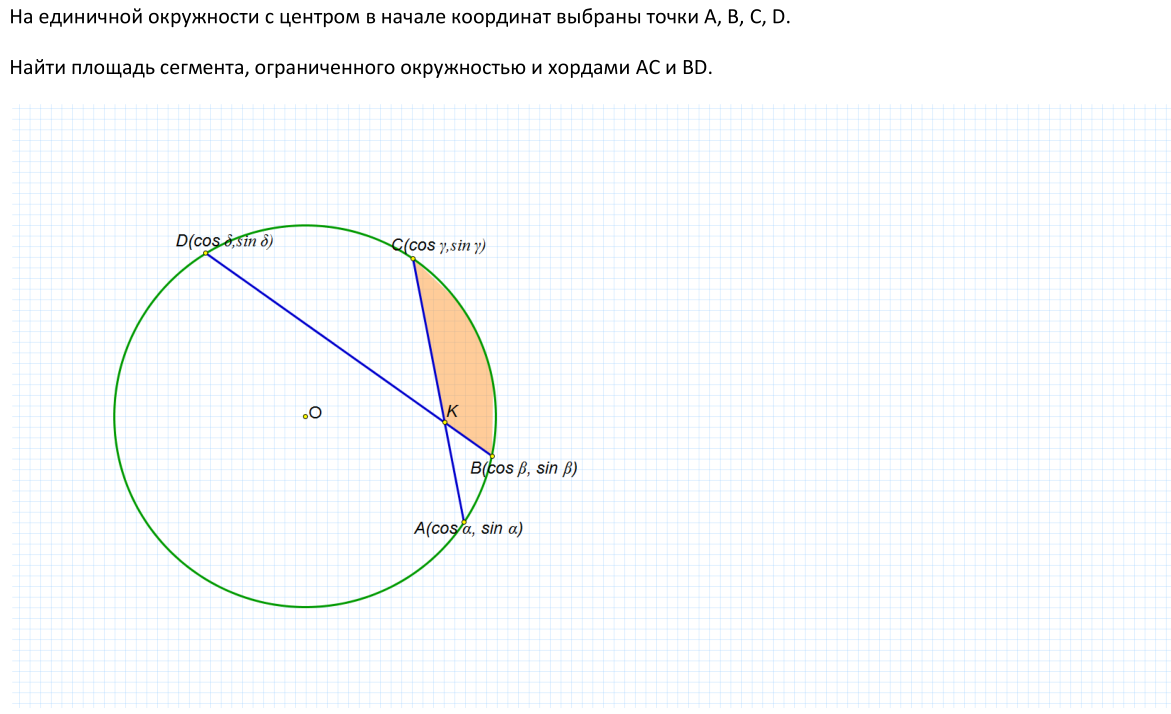
\includegraphics[width=1\linewidth]{prob_1} \\Рис. 1}
\end{figure}
\parТогда площадь фигуры CKB по формуле:
$$S_{BCK}=S_{\triangle BCK}+S_{BC}$$
\end{Lemma}
\proofname
\parВведём обозначения:
$$A = \sin \alpha-\sin\gamma$$
$$B = \cos \alpha-\sin\gamma$$
$$C = \sin \delta-\sin\beta$$
$$D = \cos \delta-\cos\beta$$
$$E = \sin \beta-\sin\gamma$$
$$F = \cos \beta-\cos\gamma$$
$$M = {(EDB + AD\cos \gamma - CB\cos \beta) \over (AD - CB)}$$
$$p = {1\over 2}(\sqrt{F^2-E^2} + |\cos\beta+\cos\gamma-2M|\sqrt{(1+({C\over D})^2})$$
$$p_{\triangle BCO} = {1\over 2}(2+\sqrt{F^2-E^2})$$
$$S_{\triangle BCO} = \sqrt{p_{\triangle BCO}{(p_{\triangle BCO}-1)}^2(p_{\triangle BCO}-\sqrt{F^2-E^2})}$$
Таким образом:
$$S_{\triangle BCK} = \sqrt{p(p-\sqrt{F^2-E^2})(p-|\cos\beta-M|\sqrt{(1+({C\over D})^2)})(p-|\cos\gamma-M|\sqrt{(1+({C\over D})^2)})}$$
$$S_{BC} = R^2\arcsin{(\frac{c}{2R})}-\frac{c}{4}\sqrt{4R^2-c^2},$$ где $R-\;$радиус окружности.
\begin{Theorem}
Пусть дан бесконечный положительный ряд $P=\sum_{i=1}^\infty{s(D_i)\cdot f(\ell(\xi_i))}$. Тогда $\forall\epsilon_1>0\;\exists N(\epsilon_1)$, что при $i>N$
$$\Big\vert\sum_{i=N+1}^\infty{s(D_i)\cdot f(\ell(\xi_i))}\Big\vert<\epsilon_1$$
\end{Theorem}
\proofname
\parСм. раздел 6.1
\begin{Theorem}
Пусть даны два конечных положительных ряда $P_N$ и $Q_N$ такие, что:
$$P_N=\sum_{i=1}^N{s(D_i)\cdot f(\zeta_i)},\;Q_N=\sum_{i=1}^N{s(D_i)\cdot f(R_i)}$$
где $\zeta_i\in D_i$ - произвольное
\parТогда существует такое $\epsilon_2>0$, что выполнено следующее:
$$|P_N-Q_N|<\epsilon_2$$
\end{Theorem}
\proofname
\parСм. раздел 6.2
\begin{Corollary}
Общая погрешность $\epsilon$ алгоритма решения поставленной задачи равна:$$\epsilon=\epsilon_1+\epsilon_2$$
\end{Corollary}
\section{Эллипсы рассеяния}
{\it Определение: Общее уравнение семейства эллипсов будет иметь вид\/}
$${(x-\mu_x)^2\over \sigma_1^2} - {2\cdot \rho\cdot x\cdot y\over \sigma_1\cdot \sigma_2} + {(y-\mu_y)^2\over \sigma_2^2} = \it{const}$$

В рассматриваемом двумерном случае выберем в качестве геометрической модели рассмотрим так называемые эллипсы рассеяния, которые получаются при проецировании на плоскость $xOy$ сечений кривой Гаусса, параллельных оси $Ox$
\begin{figure}[h]
\begin{minipage}[h]{0.49\linewidth}
\center{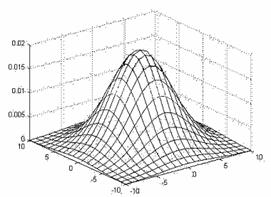
\includegraphics[width=1\linewidth]{gaussian} \\Рис. 2 Гауссиан}
\end{minipage}
\begin{minipage}[h]{0.49\linewidth}
\center{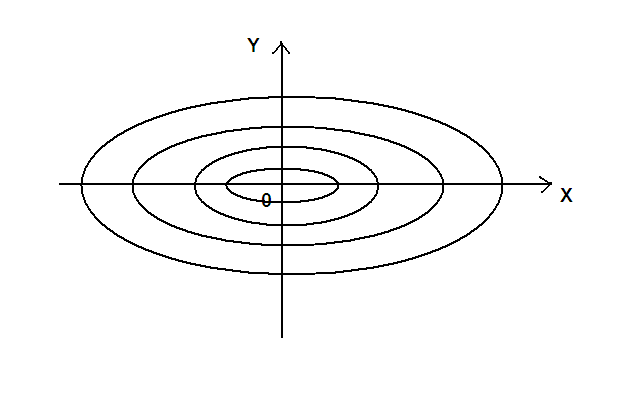
\includegraphics[width=1\linewidth]{ellipses} \\Рис.3 Эллипсы рассеяния}
\end{minipage}
\end{figure}
По условию, матрица ковариаций имеет вид:
$$ K = \left( 
\begin{matrix}
\sigma_1^2 & \rho\cdot\sigma_1\cdot\sigma_2 \\ \rho\cdot\sigma_1\cdot\sigma_2 & \sigma_2^2
\end{matrix}
\right),$$
где $\sigma_1$ и $\sigma_2$ - дисперсии, а $\rho$ - коэффициент корреляции.
В общем случае, главные оси симметрии семейства эллисов образуют с осью $Ox$ угол $\alpha_i, i =\{1,2\}$, тангенс которого определяется по следующей формуле:
$$\tg2\alpha_i={ 2\cdot \rho\cdot \sigma_1\cdot \sigma_2\over \sigma_1^2 - \sigma_2^2}$$
Вычисление площади участка, ограниченного осями координат и графиком очередного эллипса - задача трудоёмкая, поэтому воспользуемся оператором аффинного преобразования - оператором сжатия, применим его к всему семейству эллипсов и в результате получим семейство окружностей.
\begin{figure}[h!]
\begin{minipage}[h!]{0.49\linewidth}
\center{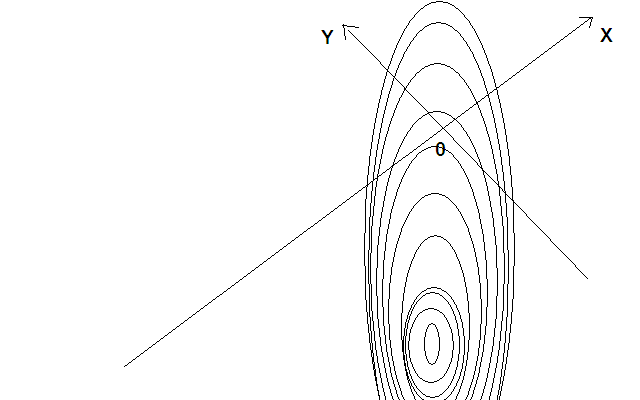
\includegraphics[width=1\linewidth]{cut} \\Рис.4 Эллипсы рассеяние исходной задачи}
\end{minipage}
\begin{minipage}[h!]{0.49\linewidth}
\center{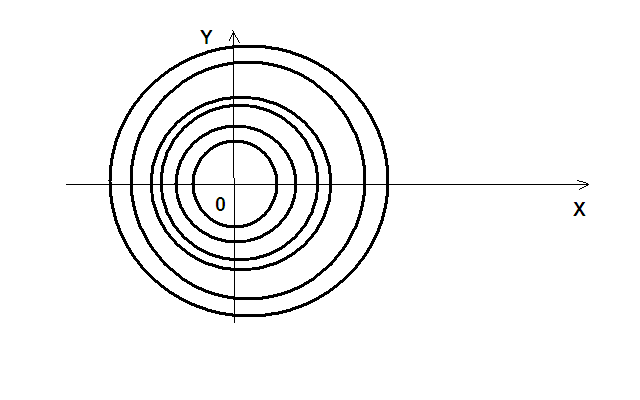
\includegraphics[width=1\linewidth]{circ_fam} \\Рис. 5 Эллипсы рассеяния после смещения, поворота и сжатия(семейство окружностей)}
\end{minipage}
\end{figure}
\parДля того, чтобы найти площадь участка, ограниченного осями координат и графиком окружности, решим следующую общую задачу, представленную на рис. 1.
\parПлощадь необходимой нам фигуры, заключенной между дугой $\breve{BC}$ и 2-мя пересекающимися хордами, есть сумма площади треугольника $\triangle${\it BCK}($S_{\triangle BCK}$), и кругового сегмента хорды {\it BC} и дуги $\breve{BC}$($S_{BC}$).
\section{Аппроксимация интеграла с помощью бесконечной  суммы}
\parКак указано в разделе ''Постановка задачи'', полная вероятность попадания произвольной точки равна:
 $$P = \iint\limits_{x\in R^n_+}p(x,y)dxdy.$$
\parСогласно избранному методу решения задачи с помощью семейства эллипсов рассеяния, полная вероятность принимает вид:
 $$P = \sum_{i=1}^\infty\int\limits_{D_i}p(x,y)\ dxdy,$$
 где $D_i$ = $\{(x,y)\in R^{+}|R_i<l(x,y)\le R_{i+1}\}$.
\parТак как функция $p(x,y)$ интегрируема в области $D_i$, и выполнено неравество $\frac{1}{\sqrt{4\pi^2detK}}\exp\{-\frac{1}{2}R_{i+1}\}\le{p(x,y)}\le \frac{1}{\sqrt{4\pi^2detK}}\exp\{-\frac{1}{2}R_{i}\}$, воспользуемся теоремой о среднем и получим:
$$P = \sum_{i =1}^\infty s(D_i)\cdot f(\ell(\xi_i)),$$
\parПусть $\ell(\xi_i)=\zeta_i$. Получаем:
$$p(x) = \frac{1}{\sqrt{4\pi^2detK}}e^{-\frac{1}{2}(x-\mu)K^{-1}(x-\mu)^{T}}\Rightarrow f(\zeta_i) = \frac{1}{\sqrt{4\pi^2detK}}e^{-\frac{1}{2}\zeta_i}$$
\parПроизводная от $f(\zeta_i)$ равна:
$$f'(\zeta_i) = -\frac{1}{2\sqrt{4\pi^2detK}}e^{-\frac{1}{2}\zeta_i}$$
\parЗафиксируем на области $D_i$ точку $\tilde{\zeta}$ и рассмотрим сумму вида
$$P_N = \sum_{i =1}^N s(D_i)\cdot f(\tilde{\zeta}),$$
где $N = N(\epsilon)$, $\epsilon$ - верхняя оценка остатка ряда $P$ в процессе аппроксимации.
\parДанный ряд показывает возможность реализации подсчёта вероятности по данным задачи на ЭВМ. Для организации конечного времени вычислений, необходимо задавать порог, при котором значение вероятности $P$ бесконечно мало, т.е. задать точность $\epsilon$.
\parВ данном случае искомая величина $\epsilon$ будет суммой двух видов погрешности: $\epsilon_1$(погрешность аппроксимации бесконечной суммы ряда, задаваемая как верхняя оценка остатка этого ряда), и $\epsilon_2$(погрешность при фиксировании точки на области $D_i$)
 \section{Оценка погрешностей}
	\subsection{Оценка сверху остатка бесконечного ряда $P$}
Для оценки погрешности аппроксимации, воспользуемся преобразованием Абеля и применим его к приближенной формуле вычисления вероятности.
Оценим $r_n$-тый остаток приближенной формулы вычисления вероятности. По формуле преобразования Абеля получаем:
$$\sum_{i=n+1}^{\infty}s(D_i)f(\zeta_{i})\Rightarrow \lim_{A \to \infty}\left|\sum_{i=n+1}^{A}s(D_i)f(\zeta_{i})\right|$$
$$\Rightarrow \lim_{A \to \infty}\left|(f(\zeta_A)s(D_A) - \sum_{i=n+1}^{A-1}\big(f(\zeta_{i+1})-f(\zeta_i)\big)H_i)\right|,$$где $H_i=\sum_{m=0}^i{s(D_m)}$ -- положим ограниченная числовая последовательность, $|H_i|\le L$, где $L=const,\;L>0$
\parИсходя из вида функции $f(\zeta_A)$, при $\lim_{A \to \infty}f(\zeta_A)\rightarrow 0$, а $s(D_A)$ - величина конечная и, следовательно, ограниченная. Получаем:
$$\lim_{A\to\infty}\left|\sum_{i=n+1}^{A-1}{\big(f(\zeta_{i+1})-f(\zeta_i)\big)H_i}\right|$$
\parРассмотрим график функции $f(x),\;0\le x\le+\infty$
\begin{figure}[h]
\center{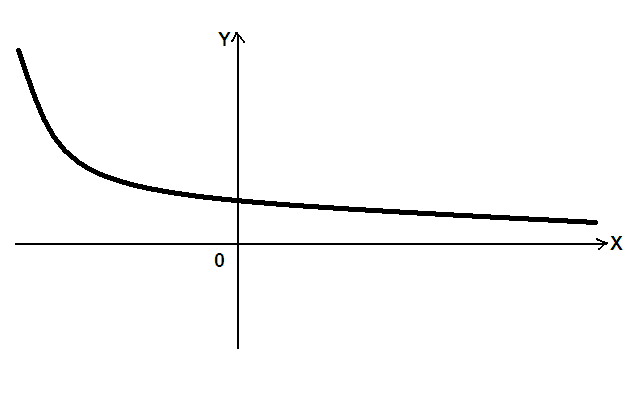
\includegraphics[width=1\linewidth]{act_gauss} \\Рис. 6 График функции $f(x),\;0\le x\le+\infty$}
\end{figure}
\parИз рисунка видно, что при $x\to+\infty:\;f(x)\to0$. Следовательно $\exists\tilde{\epsilon}>0$, что $\sum_{i=n+1}^\infty|f(\zeta_{i+1})-f(\zeta_i)|<\tilde{\epsilon}$. Т.к. $|H_i|<L$, то положим значение $\tilde{\epsilon}=\frac{\epsilon_1}{L}$. Получим:
$$\lim_{A\to\infty}\left|\sum_{i=n+1}^{A-1}{\big(f(\zeta_{i+1})-f(\zeta_i)\big)H_i}\right|<\frac{\epsilon_1}{L}\cdot L=\epsilon_1$$ 
\subsection{Оценка сверху погрешности вычисления интеграла на слое эллипсоида}
\parПри рассмотрении вида двумерного гауссиана, удовлетворяющего данным задачи, становится видно, что график гауссиана, со значенияями абсциссы из первого квадранта, представляет собой бесконечно убывающую функцию. Эта функция обозначена как $f(x), 0 \le x \le +\infty$.
\parПри выводе ряда аппроксимации $P_N$ была предварительно зафиксирована произвольная точка на области $D_i$. Для получения верхней оценки погрешности такой фиксации воспользуемся свойством бесконечного убывания графика функции $f(x)$.
\parИтак, зафиксируем точку $\zeta_i$ на области $D_i$ 
\parТ.к. выполнено $R_i \le \zeta_i \le R_{i+1}$, то $f(R_i)\ge f(\zeta_i)\ge f(R_{i+1})$. Исходя из намерения получить верхнюю оценку, то выберем в качестве $f(\zeta_i) = max\{f(R_i),f(R_{i+1})\}$. Получим
$$Q_N=\sum_{i=1}^Ns(D_i)f(R_i)$$
\parТеперь, зная $Q_N$, задача состоит в оценке следующего выражения:
$$\vert P_N-Q_N\vert=	\sum_{i=1}^Ns(D_i)(f(R_i) - f(\tilde{\zeta}))$$
\parТ.к. $D_i$ представляет собой конечную область, то и площадь этой области будет конечной, соответственно ряд $\sum_{i=1}^N{s(D_i)}$ является ограниченным некоторым наперед заданным числом $L>0$. Таким образом:
$$\vert P_N-Q_N\vert<L\vert\sum_{i=1}^N{f(R_i) - f(\tilde{\zeta})}\vert$$ 
Обращая внимание на рис. 7, видно, что часть графика, попадающего в первый квадрант, представляет непрерывную бесконечно убывающую функцию. Следовательно, существует такое $\tilde{\epsilon}=\frac{\epsilon_2}{L}>0$, что выполнено:
$$L\vert\sum_{i=1}^N{f(R_i) - f(\tilde{\zeta})}\vert\le L\cdot\tilde{\epsilon}=L\cdot\frac{\epsilon_2}{L}=\epsilon_2$$ 
\begin{figure}[h]
\begin{minipage}[h]{0.49\linewidth}
\center{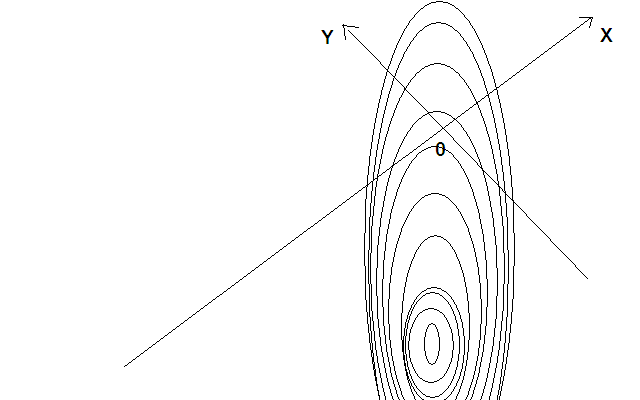
\includegraphics[width=1\linewidth]{cut} \\Рис.7 Разрез трехмерного гауссиана на эллипсы рассеяния}
\end{minipage}
\begin{minipage}[h]{0.49\linewidth}
\center{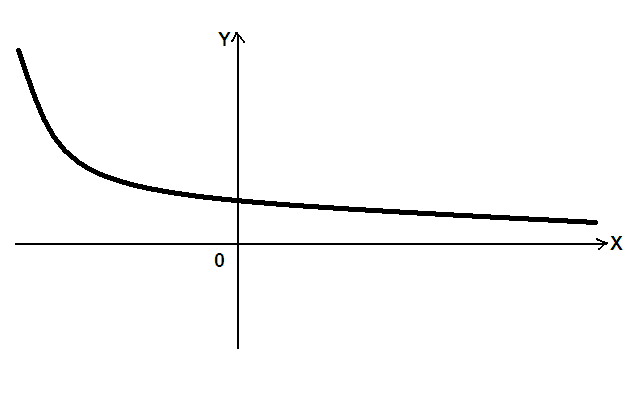
\includegraphics[width=1\linewidth]{act_gauss} \\Рис. 8 Часть гауссиана, попадающая в первый октант}
\end{minipage}
\end{figure}
\section{Выводы}
\parПриведена математическая модель решения поставленной задачи - построение семейства эллипсов рассеяния. Получено решение поставленной задачи посредством вычисления площадей областей, расположенных между соседними эллипсов и их последующем суммировании. Доказана аппроксимация бесконечного интеграла $P$ конечной суммой $P_N$. Проведена оценка погрешности данной аппроксимации. Решение задачи реализовано в виде MFC-приложения.
\begin{thebibliography}{2}
\item
Александров П.С. \emph{Курс аналитической геометрии и линейной алгебры} - М.: Наука, Главная редакция физико-математической литературы, 1979
\item
Вентцель Е.С. \emph{Теория вероятностей: Учеб. для вузов., 6-е изд. стер.} - М.: Высш. шк., 1999
\item
D.R.Cox, N. Wermuth \emph{A Simple Approximation for Bivariate and Trivariate Normal Integrals} - International Statistical Review (1991), 59, 2, pp. 263-269
\item
Alan Genz \emph{Numerical Computation of Multivariate Normal Probabilities} - Journal of Computational and Graphical Statistics, vol.1, No. 2, Jun., 1992
\item
Alan Genz, Koon-Sing Kwong \emph{Numerical Evaluation of Singular Multivariate Normal Distributions} - revised version published in J. Stat. Comp. Simul. 68 (2000), pp. 1-21. 
\end{thebibliography}
\end{document}